\section{Additional Results}
\label{app:results}

This appendix reports the detailed results behind the summaries in Section~\mref{sec:results}. All values are generated from the simulation output by the scripts in the repository; the files in the \texttt{paper/supplement} folder contain the same results in machine-readable form.

\subsection{Face Validity}
\label{app:res:face}

Table~\ref{tab:face} gives the time intervals of the community, pooled ED under the default policy at the three load levels, which Section~\mref{sec:res:vv} compares with published Canadian values.

\begin{table}[!ht]
\centering
\caption{Face validity: community ED, pooled configuration, default policy, \Reps{} replications per load level.}
\label{tab:face}
\footnotesize
\begin{adjustbox}{max width=\linewidth}\begin{tabular}{lrrr}
\toprule
Measure (h unless stated) & Low & Medium & High \\
\midrule
Door to physician, median & 0.2 & 0.2 & 0.4 \\
Door to physician, P90 & 0.4 & 0.8 & 3.4 \\
LOS discharged, median & 1.5 & 1.6 & 2.1 \\
LOS discharged, P90 & 3.2 & 3.7 & 6.2 \\
LOS CTAS 4, P90 & 3.5 & 4.7 & 8.9 \\
LOS admitted, median & 4.9 & 5.1 & 5.4 \\
LOS admitted, P90 & 9.1 & 9.4 & 10.3 \\
Physician utilisation & 0.70 & 0.80 & 0.90 \\
Space utilisation & 0.54 & 0.67 & 0.85 \\
\bottomrule
\end{tabular}\end{adjustbox}
\end{table}

\subsection{Best Policy by ED Type}
\label{app:res:best}

Table~\ref{tab:best} lists, for every core ED type, the default policy and the best policy for RATP and mean LOS, with the number of policies that are statistically tied with the best. Table~\ref{tab:kpis} and Fig.~\ref{fig:tails} give the full set of measures for one ED type, the community ED at high load.

\begin{table*}[!t]
\centering
\caption{Default policy and best policy by ED type (\Reps{} replications). Tied: number of policies whose paired difference from the best is not significant at the 95\% level, out of all policies for the configuration.}
\label{tab:best}
\scriptsize
\setlength{\tabcolsep}{3pt}
\begin{adjustbox}{max width=\linewidth}\begin{tabular}{lllrlrr lrr}
\toprule
 & & & \multicolumn{4}{c}{RATP} & \multicolumn{3}{c}{Mean LOS (min)} \\
\cmidrule(lr){4-7}\cmidrule(lr){8-10}
Acuity & Load & Config. & Default & Best policy & Best & Tied & Best policy & Best & Default \\
\midrule
Tertiary & low & Pooled & 0.38 & SIM & 0.36 & 1/7 & FCFS & 154 & 155 \\
 &  & Fast track & 0.44 & SIM/S & 0.38 & 5/21 & FCFS/S & 154 & 155 \\
 &  & Split flow & 0.37 & SIM/S & 0.35 & 2/21 & FCFS/C & 154 & 155 \\
\addlinespace[1pt]
 & medium & Pooled & 0.60 & SIM & 0.53 & 1/7 & SIM & 166 & 168 \\
 &  & Fast track & 0.64 & SIM/S & 0.50 & 1/21 & FCFS/S & 162 & 168 \\
 &  & Split flow & 0.58 & SIM/S & 0.50 & 1/21 & FCFS/S & 165 & 167 \\
\addlinespace[1pt]
 & high & Pooled & 1.09 & SIM & 0.89 & 1/7 & SIM & 204 & 229 \\
 &  & Fast track & 1.02 & SIM/S & 0.76 & 1/21 & SIM/S & 179 & 203 \\
 &  & Split flow & 0.96 & SIM/S & 0.80 & 2/21 & SIM-AGE/S & 193 & 206 \\
\addlinespace[1pt]
Community & low & Pooled & 0.38 & CTAS-PD & 0.37 & 5/7 & FCFS & 138 & 138 \\
 &  & Fast track & 0.55 & SIM/S & 0.47 & 1/21 & SIM/C & 143 & 144 \\
 &  & Split flow & 0.37 & CTAS-SPT/S & 0.36 & 3/21 & FCFS/S & 138 & 138 \\
\addlinespace[1pt]
 & medium & Pooled & 0.60 & SIM & 0.56 & 1/7 & SIM & 151 & 155 \\
 &  & Fast track & 0.83 & SIM/S & 0.65 & 1/21 & SIM/C & 157 & 159 \\
 &  & Split flow & 0.59 & CTAS-SPT/S & 0.53 & 3/21 & SIM/S & 150 & 154 \\
\addlinespace[1pt]
 & high & Pooled & 1.05 & SIM & 0.92 & 1/7 & SIM & 195 & 213 \\
 &  & Fast track & 1.31 & SIM/S & 1.07 & 1/21 & SIM/S & 199 & 212 \\
 &  & Split flow & 0.96 & CTAS-SPT/S & 0.84 & 3/21 & FCFS/S & 187 & 202 \\
\addlinespace[1pt]
Urgent-care-like & low & Pooled & 0.30 & CTAS & 0.30 & 3/7 & SIM & 119 & 120 \\
 &  & Fast track & 0.77 & SIM/S & 0.53 & 5/21 & FCFS/S & 126 & 128 \\
 &  & Split flow & 0.41 & CTAS/S & 0.37 & 5/21 & SIM/S & 120 & 120 \\
\addlinespace[1pt]
 & medium & Pooled & 0.57 & CTAS-SPT & 0.55 & 4/7 & SIM & 130 & 135 \\
 &  & Fast track & 1.15 & SIM/S & 0.83 & 2/21 & SIM/S & 140 & 149 \\
 &  & Split flow & 0.68 & CTAS/S & 0.63 & 4/21 & FCFS/S & 131 & 134 \\
\addlinespace[1pt]
 & high & Pooled & 0.92 & CTAS-SPT & 0.87 & 3/7 & SIM & 165 & 192 \\
 &  & Fast track & 1.55 & CTAS-SPT/S & 1.28 & 4/21 & SIM/S & 189 & 223 \\
 &  & Split flow & 1.00 & CTAS-SPT/C & 0.93 & 5/21 & FCFS/S & 163 & 172 \\
\bottomrule
\end{tabular}\end{adjustbox}
\end{table*}

\begin{table*}[!ht]
\centering
\caption{Performance by queue rule in the community ED at high load (pooled; \Reps{} replications). Second line of each measure: paired difference from CTAS; bold if the 95\% confidence interval excludes zero.}
\label{tab:kpis}
\footnotesize
\begin{adjustbox}{max width=\linewidth}\begin{tabular}{lrrrrrrr}
\toprule
KPI & FCFS & CTAS & APQ & CTAS-SPT & CTAS-PD & SIM & SIM-AGE \\
\midrule
RATP & 1.145 & 1.046 & 1.177 & 0.982 & 1.009 & 0.918 & 1.031 \\
\quad vs CTAS & \textbf{+0.099} & -- & \textbf{+0.130} & \textbf{-0.064} & \textbf{-0.037} & \textbf{-0.128} & -0.015 \\
AWT (min) & 48.3 & 89.2 & 54.6 & 85.6 & 89.9 & 50.1 & 49.8 \\
\quad vs CTAS & \textbf{-41.0} & -- & \textbf{-34.6} & \textbf{-3.6} & +0.6 & \textbf{-39.1} & \textbf{-39.4} \\
P90 door to physician (min) & 147 & 206 & 164 & 152 & 185 & 102 & 150 \\
\quad vs CTAS & \textbf{-59} & -- & \textbf{-42} & \textbf{-53} & \textbf{-20} & \textbf{-104} & \textbf{-56} \\
P95 door to physician, CTAS 2 (min) & 194 & 31 & 86 & 31 & 31 & 101 & 77 \\
\quad vs CTAS & \textbf{+163} & -- & \textbf{+55} & -0 & +0 & \textbf{+70} & \textbf{+46} \\
P95 door to physician, CTAS 5 (min) & 188 & 1289 & 594 & 1328 & 1320 & 654 & 700 \\
\quad vs CTAS & \textbf{-1101} & -- & \textbf{-695} & +39 & +31 & \textbf{-635} & \textbf{-589} \\
Mean LOS (min) & 197.7 & 212.9 & 203.3 & 207.5 & 211.9 & 195.0 & 196.0 \\
\quad vs CTAS & \textbf{-15.2} & -- & \textbf{-9.6} & \textbf{-5.5} & \textbf{-1.0} & \textbf{-18.0} & \textbf{-16.9} \\
Mean LOS, discharged (min) & 160.9 & 184.1 & 170.2 & 176.8 & 179.7 & 146.3 & 156.8 \\
\quad vs CTAS & \textbf{-23.3} & -- & \textbf{-14.0} & \textbf{-7.3} & \textbf{-4.4} & \textbf{-37.8} & \textbf{-27.3} \\
Mean LOS, admitted (min) & 412.6 & 381.2 & 396.9 & 386.4 & 399.8 & 478.7 & 424.8 \\
\quad vs CTAS & \textbf{+31.4} & -- & \textbf{+15.7} & \textbf{+5.3} & \textbf{+18.7} & \textbf{+97.5} & \textbf{+43.6} \\
\bottomrule
\end{tabular}\end{adjustbox}
\end{table*}

\begin{figure}[!ht]
\centering
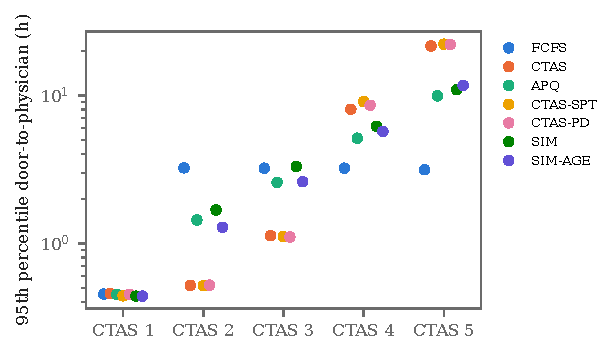
\includegraphics[width=0.95\columnwidth]{figures/fig_tails.pdf}
\caption{95th percentile of door-to-physician time by CTAS level and queue rule (community ED, high load, pooled; log scale).}
\label{fig:tails}
\end{figure}

\subsection{How Firmly Is the Best Policy Identified?}
\label{app:res:boot}

For each ED type and measure we drew \BootB{} bootstrap samples of the \Reps{} replications (resampling replications, so that the pairing of policies on common random numbers is kept) and recorded which policy had the lowest mean in each sample. For RATP the policy that is best on the full sample remains best in a median of \BootRatpMedianP\% of the bootstrap samples; the share is at least 90\% in \BootRatpNNinety{} of the \NEdTypes{} ED types and below one half in \BootRatpNHalf. For mean LOS the median is \BootLosMedianP\% (at least 90\% in \BootLosNNinety{} ED types, below one half in \BootLosNHalf). Where the share is low, two or more policies are practically equivalent, which is consistent with the ties reported in Table~\ref{tab:best}; the regret of choosing any of them is then small.

\subsection{Alternative Acuity Weights in RATP}
\label{app:res:altw}

RATP weights the breach rate of CTAS level $l$ by $1/l$. Table~\ref{tab:altw} repeats the identification of the best policy per ED type and of the best single policy with three other weightings. With linear weights $6-l$, the best policy is unchanged in \AltWLinearSame{} of the \NEdTypes{} ED types; with equal weights in \AltWEqualSame{}; and with inverse-square weights in \AltWSteepSame. Equal weights give the breach rate of all patients and therefore put most weight on CTAS~3 and~4, which are the largest groups.

\begin{table}[!t]
\centering
\caption{Best policies under alternative acuity weights for the breach-rate measure. Same best: number of ED types in which the best policy equals the best policy under RATP. Best single policy: the policy with the smallest mean regret over all ED types.}
\label{tab:altw}
\footnotesize
\begin{adjustbox}{max width=\linewidth}\begin{tabular}{lrlrr}
\toprule
Acuity weights & Same best as RATP & Best single policy & Mean regret (\%) & Max regret (\%) \\
\midrule
$1/l$ (RATP) & 27/27 & CTAS-SPT/S & 2.8 & 13.5 \\
$6-l$ & 25/27 & CTAS-SPT/S & 2.3 & 13.6 \\
equal & 18/27 & SIM/S & 1.7 & 14.5 \\
$1/l^2$ & 17/27 & CTAS-SPT/S & 1.8 & 5.3 \\
\bottomrule
\end{tabular}\end{adjustbox}
\end{table}

\subsection{Sensitivity to Boarding and Diagnostic Intensity}
\label{app:res:sens}

Table~\ref{tab:sens} reports the sensitivity analysis summarized in Section~\mref{sec:res:sens}. The supplement contains the results for every policy and ED type, and those of the value-of-prediction experiment.

\begin{table}[!ht]
\centering
\caption{Sensitivity (\NMediumTypes{} medium-load ED types, \RepsSecondary{} replications): number of ED types in which the core best policy is still best, and mean (maximum) regret of keeping the core best policy.}
\label{tab:sens}
\footnotesize
\setlength{\tabcolsep}{3pt}
\begin{adjustbox}{max width=\linewidth}\begin{tabular}{lrrrr}
\toprule
 & \multicolumn{2}{c}{RATP} & \multicolumn{2}{c}{Mean LOS} \\
\cmidrule(lr){2-3}\cmidrule(lr){4-5}
Variant & Same best & Regret of core best (\%) & Same best & Regret of core best (\%) \\
\midrule
High boarding & 5/9 & 1.0 (max 4.6) & 5/9 & 2.3 (max 12.7) \\
Light diagnostics & 6/9 & 0.5 (max 2.1) & 4/9 & 0.1 (max 0.5) \\
Heavy diagnostics & 5/9 & 5.7 (max 32.3) & 4/9 & 11.7 (max 83.0) \\
\bottomrule
\end{tabular}\end{adjustbox}
\end{table}

\subsection{Trade-Offs and Value of Prediction}
\label{app:res:vop}

Fig.~\ref{fig:pareto} shows mean LOS against RATP for all policies in the community ED at high load, and Table~\ref{tab:vop} the gain of the best prediction-based policy over the best policy without predictions in the medium-load ED types (Sections~\mref{sec:res:mech} and~\mref{sec:res:vop}).

\begin{figure}[!ht]
\centering
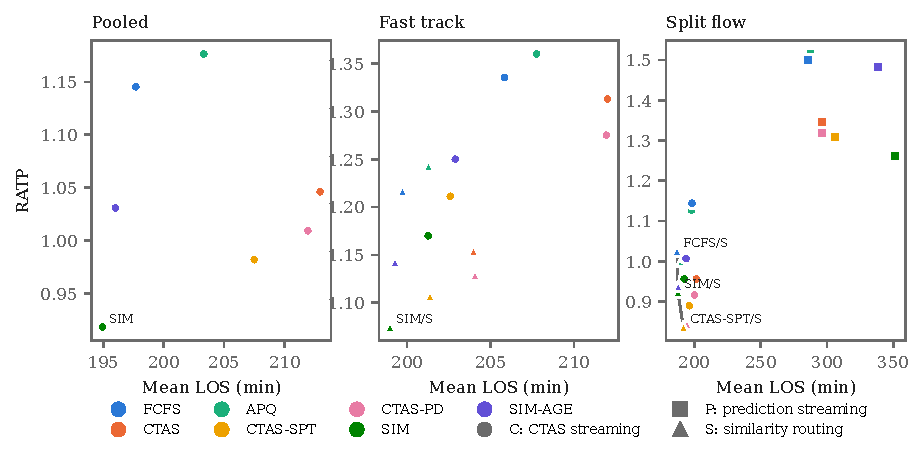
\includegraphics[width=\columnwidth]{figures/fig_pareto.pdf}
\caption{Mean LOS against RATP for all policies in the community ED at high load. Grey line: policies not dominated on both measures (labelled). Overloaded policies (Main-area utilization $\geq$ \OverloadThreshold) are omitted.}
\label{fig:pareto}
\end{figure}

\begin{table*}[!ht]
\centering
\caption{Gain of the best prediction-based policy over the best policy without predictions (medium load), with perfect information ($\alpha=0$) and reference accuracy ($\alpha=1$), and the largest $\alpha$ tested at which it is still better ($\geq$: better at every $\alpha$ tested).}
\label{tab:vop}
\footnotesize
\setlength{\tabcolsep}{2.5pt}
\begin{adjustbox}{max width=\linewidth}\begin{tabular}{llrrrrrr}
\toprule
 & & \multicolumn{3}{c}{RATP} & \multicolumn{3}{c}{Mean LOS} \\
\cmidrule(lr){3-5}\cmidrule(lr){6-8}
Acuity & Config. & Gain $\alpha{=}0$ (\%) & Gain $\alpha{=}1$ (\%) & Max $\alpha$ & Gain $\alpha{=}0$ (\%) & Gain $\alpha{=}1$ (\%) & Max $\alpha$ \\
\midrule
Tertiary & Pooled & 12.7 & 11.1 & $\geq$1.50 & 1.2 & 1.0 & $\geq$1.50 \\
 & Fast track & 23.3 & 21.5 & $\geq$1.50 & 3.6 & 3.3 & $\geq$1.50 \\
 & Split flow & 12.9 & 11.9 & $\geq$1.50 & 1.1 & 1.1 & $\geq$1.50 \\
Community & Pooled & 11.3 & 7.4 & $\geq$1.50 & 1.8 & 1.6 & $\geq$1.50 \\
 & Fast track & 21.2 & 20.9 & $\geq$1.50 & 0.8 & 0.8 & $\geq$1.50 \\
 & Split flow & 11.5 & 11.5 & $\geq$1.50 & 1.9 & 1.8 & $\geq$1.50 \\
Urgent-care-like & Pooled & 0.9 & 0.6 & 1.50 & 2.6 & 2.5 & $\geq$1.50 \\
 & Fast track & 22.4 & 25.9 & $\geq$1.50 & 2.6 & 5.0 & $\geq$1.50 \\
 & Split flow & 4.1 & 7.0 & 1.50 & 1.7 & 2.0 & $\geq$1.50 \\
\bottomrule
\end{tabular}\end{adjustbox}
\end{table*}

\subsection{Optimized Similarity Rules: Details}
\label{app:res:opt}

Table~\ref{tab:optfull} gives the test-replication objective of the default policy, the best fixed policy and the optimized similarity policy for every ED type. The best fixed policy is the one with the lowest mean objective on the same test replications, so the comparison is conservative for the optimized rule: the fixed policy is selected with knowledge of the test outcomes, the optimized rule is not. Fig.~\ref{fig:optparamsaccess} shows the parameters of the rules optimized for the access objective (Fig.~\mref{fig:optparams} in the main text shows the balanced objective) and Fig.~\ref{fig:cem} the progress of the search. On average, the training objective of the selected rule was \OptAccessTrainOptimism\% (access) and \OptBalancedTrainOptimism\% (balanced) away from its test value and the validation objective \OptAccessValOptimism\% and \OptBalancedValOptimism\%; negative values mean the search replications were more favourable than the test replications. Each search used about \CemEvalsPerType{} simulation runs per ED type and objective. Table~\ref{tab:levers} gives the lever check of experiment E6b and Fig.~\ref{fig:transfer} the transfer regret of every pair of ED types.

\begin{table*}[!t]
\centering
\caption{Objective on the \Reps{} test replications by ED type: default policy (CTAS/C), best fixed policy, and optimized similarity policy. Balanced objective: $J=\tfrac12\,\text{RATP}/\text{RATP}_0+\tfrac12\,\overline{\text{LOS}}/\overline{\text{LOS}}_0$, so $J=1$ for the default policy. $^{*}$: optimized better than the best fixed policy (paired 95\% confidence interval excludes zero); $^{\dagger}$: worse.}
\label{tab:optfull}
\scriptsize
\setlength{\tabcolsep}{3pt}
\begin{adjustbox}{max width=\linewidth}\begin{tabular}{lllrrrlrrr}
\toprule
 & & & \multicolumn{3}{c}{Access (RATP)} & \multicolumn{4}{c}{Balanced ($J$)} \\
\cmidrule(lr){4-6}\cmidrule(lr){7-10}
Acuity & Load & Config. & Default & Best fixed & Optimized & Best fixed policy & Default & Best fixed & Optimized \\
\midrule
Tertiary & low & Pooled & 0.375 & 0.359 & 0.350$^{*}$ & SIM & 1.000 & 0.977 & 0.971 \\
 &  & Fast track & 0.441 & 0.382 & 0.364$^{*}$ & SIM/S & 1.000 & 0.930 & 0.916$^{*}$ \\
 &  & Split flow & 0.372 & 0.350 & 0.331$^{*}$ & SIM/S & 1.000 & 0.970 & 0.953$^{*}$ \\
 & medium & Pooled & 0.598 & 0.532 & 0.520$^{*}$ & SIM & 1.000 & 0.938 & 0.934 \\
 &  & Fast track & 0.637 & 0.498 & 0.490 & SIM/S & 1.000 & 0.873 & 0.870 \\
 &  & Split flow & 0.576 & 0.504 & 0.436$^{*}$ & SIM/S & 1.000 & 0.931 & 0.902$^{*}$ \\
 & high & Pooled & 1.093 & 0.889 & 0.836$^{*}$ & SIM & 1.000 & 0.854 & 0.832$^{*}$ \\
 &  & Fast track & 1.023 & 0.758 & 0.733$^{*}$ & SIM/S & 1.000 & 0.813 & 0.799$^{*}$ \\
 &  & Split flow & 0.964 & 0.801 & 0.569$^{*}$ & SIM/S & 1.000 & 0.885 & 0.837$^{*}$ \\
Community & low & Pooled & 0.375 & 0.371 & 0.358$^{*}$ & CTAS-SPT & 1.000 & 0.996 & 0.984 \\
 &  & Fast track & 0.555 & 0.467 & 0.457 & SIM/S & 1.000 & 0.938 & 0.923$^{*}$ \\
 &  & Split flow & 0.372 & 0.356 & 0.326$^{*}$ & CTAS-SPT/S & 1.000 & 0.980 & 0.954$^{*}$ \\
 & medium & Pooled & 0.603 & 0.561 & 0.554 & SIM & 1.000 & 0.953 & 0.952 \\
 &  & Fast track & 0.828 & 0.654 & 0.628$^{*}$ & SIM/S & 1.000 & 0.893 & 0.887 \\
 &  & Split flow & 0.594 & 0.527 & 0.418$^{*}$ & CTAS-SPT/S & 1.000 & 0.939 & 0.872$^{*}$ \\
 & high & Pooled & 1.046 & 0.918 & 0.897 & SIM & 1.000 & 0.897 & 0.877$^{*}$ \\
 &  & Fast track & 1.313 & 1.075 & 0.999$^{*}$ & SIM/S & 1.000 & 0.879 & 0.833$^{*}$ \\
 &  & Split flow & 0.957 & 0.837 & 0.529$^{*}$ & CTAS-SPT/S & 1.000 & 0.914 & 0.777$^{*}$ \\
Urgent-care-like & low & Pooled & 0.301 & 0.301 & 0.319 & CTAS & 1.000 & 1.000 & 1.035 \\
 &  & Fast track & 0.766 & 0.532 & 0.493 & SIM/S & 1.000 & 0.839 & 0.836 \\
 &  & Split flow & 0.412 & 0.368 & 0.277$^{*}$ & CTAS/S & 1.000 & 0.960 & 0.843$^{*}$ \\
 & medium & Pooled & 0.566 & 0.547 & 0.573 & CTAS-SPT & 1.000 & 0.985 & 1.000 \\
 &  & Fast track & 1.151 & 0.828 & 0.772$^{*}$ & SIM/S & 1.000 & 0.830 & 0.817 \\
 &  & Split flow & 0.680 & 0.631 & 0.412$^{*}$ & CTAS-PD/S & 1.000 & 0.962 & 0.808$^{*}$ \\
 & high & Pooled & 0.923 & 0.874 & 0.873 & SIM & 1.000 & 0.913 & 0.903 \\
 &  & Fast track & 1.547 & 1.276 & 1.145$^{*}$ & SIM/S & 1.000 & 0.846 & 0.759$^{*}$ \\
 &  & Split flow & 1.001 & 0.930 & 0.479$^{*}$ & CTAS-SPT/C & 1.000 & 0.952 & 0.736$^{*}$ \\
\bottomrule
\end{tabular}\end{adjustbox}
\end{table*}

\begin{figure*}[!t]
\centering
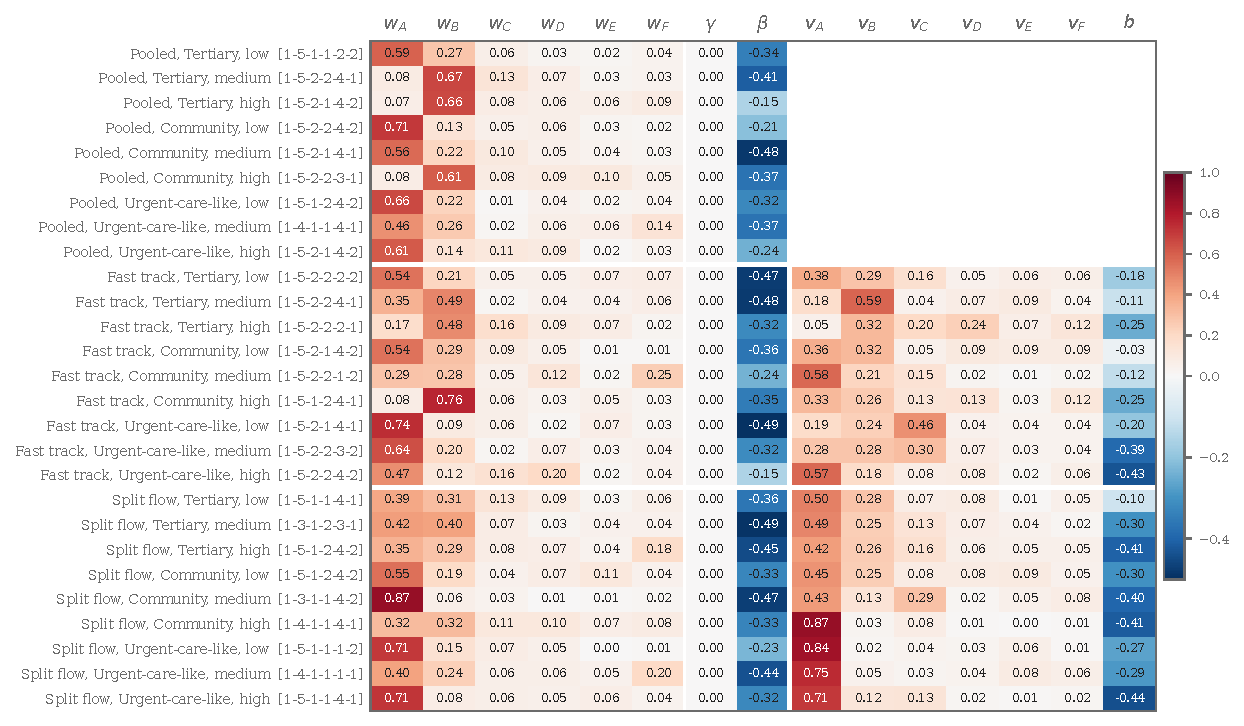
\includegraphics[width=\textwidth]{figures/fig_opt_params_access.pdf}
\caption{Parameters of the similarity rules optimized for the access objective. Rows: ED types, with the optimized target code $q_A$--$q_F$ in brackets. Columns: queue weights, ageing $\gamma$, reassessment bonus $\beta$, routing weights and routing offset $b$ (two-area EDs only).}
\label{fig:optparamsaccess}
\end{figure*}

\begin{figure}[!t]
\centering
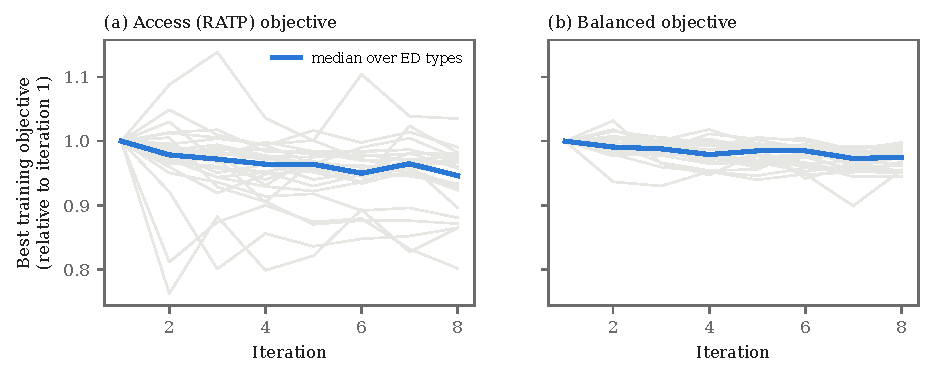
\includegraphics[width=\columnwidth]{figures/fig_cem_convergence.pdf}
\caption{Best training objective by iteration of the cross-entropy search, relative to the first iteration. Grey: individual ED types; blue: median.}
\label{fig:cem}
\end{figure}

\begin{table}[!ht]
\centering
\caption{Change in the objective (\%) when one parameter of the optimized rule is changed (E6b, \NLeverReps{} test replications); negative is better. Better/worse: ED types with a change of more than 1\% in either direction.}
\label{tab:levers}
\footnotesize
\begin{adjustbox}{max width=\linewidth}\begin{tabular}{lrrrrrr}
\toprule
 & \multicolumn{3}{c}{Access objective} & \multicolumn{3}{c}{Balanced objective} \\
\cmidrule(lr){2-4}\cmidrule(lr){5-7}
Change to the optimized rule & Mean change (\%) & Better & Worse & Mean change (\%) & Better & Worse \\
\midrule
Ageing $\gamma=0.02$ & +2.0 & 4/27 & 11/27 & +0.6 & 4/27 & 6/27 \\
Ageing $\gamma=0.05$ & +4.3 & 2/27 & 18/27 & +1.4 & 3/27 & 13/27 \\
Ageing $\gamma=0.1$ & +7.9 & 2/27 & 22/27 & +3.2 & 3/27 & 18/27 \\
Ageing $\gamma=0.2$ & +11.3 & 2/27 & 23/27 & +4.5 & 1/27 & 19/27 \\
Ageing $\gamma=0.4$ & +14.6 & 0/27 & 24/27 & +6.5 & 2/27 & 22/27 \\
No reassessment bonus ($\beta=0$) & +6.1 & 1/27 & 22/27 & +0.4 & 4/27 & 12/27 \\
No routing offset ($b=0$) & +4.4 & 4/18 & 12/18 & +2.6 & 2/18 & 7/18 \\
\bottomrule
\end{tabular}\end{adjustbox}
\end{table}

\begin{figure*}[!ht]
\centering
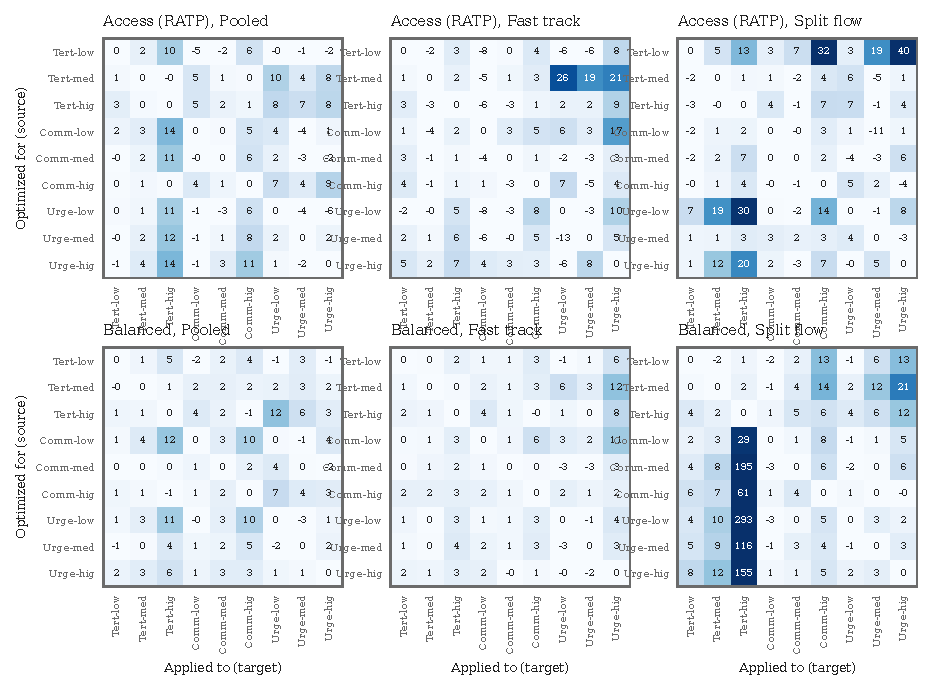
\includegraphics[width=0.95\textwidth]{figures/fig_transfer.pdf}
\caption{Transfer regret (\%) of optimized rules (\NTransferReps{} test replications). Row: ED type for which the rule was optimized; column: ED type to which it is applied; the diagonal is zero by definition. Top: access objective; bottom: balanced objective.}
\label{fig:transfer}
\end{figure*}

\subsection{Robustness to Misspecified Inputs: Details}
\label{app:res:rob}

Table~\ref{tab:rob} reports, for each perturbation in E8, the rank correlation between the policy ranking under the perturbed inputs and the ranking in the core design, the regret of the policy that was best in the core design when it is used under the perturbed inputs, and the balanced objective of the optimized rule relative to the best fixed policy under the perturbed inputs and to the default. Values are averages over the nine medium-load ED types.

\begin{table*}[!t]
\centering
\caption{Robustness of the policy ranking to misspecified inputs (medium-load ED types, \NRobReps{} replications). Kendall $\tau$: rank correlation of mean RATP or mean LOS over all fixed policies between the perturbed and the core inputs. Regret of core best: regret under the perturbed inputs of the policy that is best under the core inputs. Optimized (balanced): balanced objective of the rule optimized under the core inputs, relative to the best fixed policy under the perturbed inputs (positive: worse) and improvement over the default.}
\label{tab:rob}
\footnotesize
\begin{adjustbox}{max width=\linewidth}\begin{tabular}{lrrrrrr}
\toprule
 & \multicolumn{2}{c}{Kendall $\tau$ of policy ranking} & \multicolumn{2}{c}{Regret of core best (\%)} & \multicolumn{2}{c}{Optimized (balanced)} \\
\cmidrule(lr){2-3}\cmidrule(lr){4-5}\cmidrule(lr){6-7}
Perturbation & RATP & LOS & RATP & LOS & vs best fixed (\%) & vs default (\%) \\
\midrule
Physician times $-10\%$ & 0.85 & 0.89 & 1.3 & 0.0 & -3.0 & 9.6 \\
Physician times $+10\%$ & 0.84 & 0.81 & 0.5 & 0.6 & -2.8 & 12.5 \\
Diagnostic times $-25\%$ & 0.83 & 0.70 & 0.9 & 0.1 & -0.9 & 8.2 \\
Diagnostic times $+25\%$ & 0.84 & 0.80 & 3.0 & 0.7 & -7.7 & 17.9 \\
All CVs $\times0.5$ & 0.86 & 0.90 & 1.1 & 0.0 & -3.3 & 12.5 \\
All CVs $\times1.5$ & 0.85 & 0.88 & 1.5 & 0.1 & -3.1 & 10.8 \\
Flat arrival profile & 0.75 & 0.64 & 1.9 & 0.8 & -0.5 & 7.0 \\
Peaked arrival profile & 0.87 & 0.87 & 1.7 & 0.2 & -5.1 & 14.2 \\
Correlated prediction errors & 0.84 & 0.89 & 2.5 & 0.3 & -2.7 & 9.8 \\
\bottomrule
\end{tabular}\end{adjustbox}
\end{table*}
